\chapter{Conexión local con la BD por defecto} \label{cap:03ConexLocal}

En ocasiones, puede resultar interesante acceder a la base de datos remota de Broadsea desde un administrador de bases de datos local.  Docker almacena las bases de datos que utilizan los contenedores en lo que se denominan \textit{''volúmenes''}. Para revisar los volúmenes que están ejecutándose en el equipo se presentan dos estrategias:

\section{Requisitos para establecer la conexión}

\begin{enumerate}

    \item Descargar e instalar la base de datos PostgreSQL. Lo más sencillo es seguir las instrucciones de la \href{https://www.postgresql.org/download/}{página web oficial} para la descarga y seguir la configuración por defecto para la instalación.

    \item Descargar e instalar una administrador de base de datos PostgreSQL. Se recomienda utilizar el administrador pgAdmin. Para ello, lo más sencillo es seguir las instrucciones de la \href{https://www.pgadmin.org/download/}{página web oficial} para la descarga y seguir la configuración por defecto para la instalación.
    
\end{enumerate}


\section{Deployment}

Para establecer la conexión con la base de datos que utiliza Broadsea, se debe seguir las siguientes instrucciones:

\begin{enumerate}

    \item En primer lugar, se debe comprobar los parámetros de configuración de la base de datos. Para ello, se han detallado varias estrategias a lo largo del manual, siendo la más recomendada para esta ocasión revisar el \textit{docker-compose.yml} (Figura \ref{fig:dockerComposeDB}). Este archivo alberga la información técnica de los contendores que ejecuta Docker. En este caso, el contenedor que interesa es \textit{''broadsea-atlasdb''}.

    En el archivo por defecto, se presenta la contraseña para acceder a la base de datos \textit{(password=mypass)} y el puerto que utiliza (\textit{port=5432}).

    \item La configuración por defecto de Broadsea se solapa con la configuración local por defecto de PostgreSQL porque ambos alojan sus bases de datos en el servidor local y en el puerto 5432. Por tanto, para evitar este solapamiento se debe detener el servicio local de PostgreSQL, de forma que el puerto quede libre para albergar la base de datos de Broadsea.

    Para detener el servicio local de PostgreSQL lo más sencillo es abrir la aplicación \textit{servicios} buscar el servidor de postgre y deterlo, tal y como se muestra en la Figura \ref{fig:serviciosConfig}. Así nos aseguramos de liberar el puerto para que pueda ser ocupado por la base de datos de Broadsea.

    \begin{figure}[H]
    \centering
    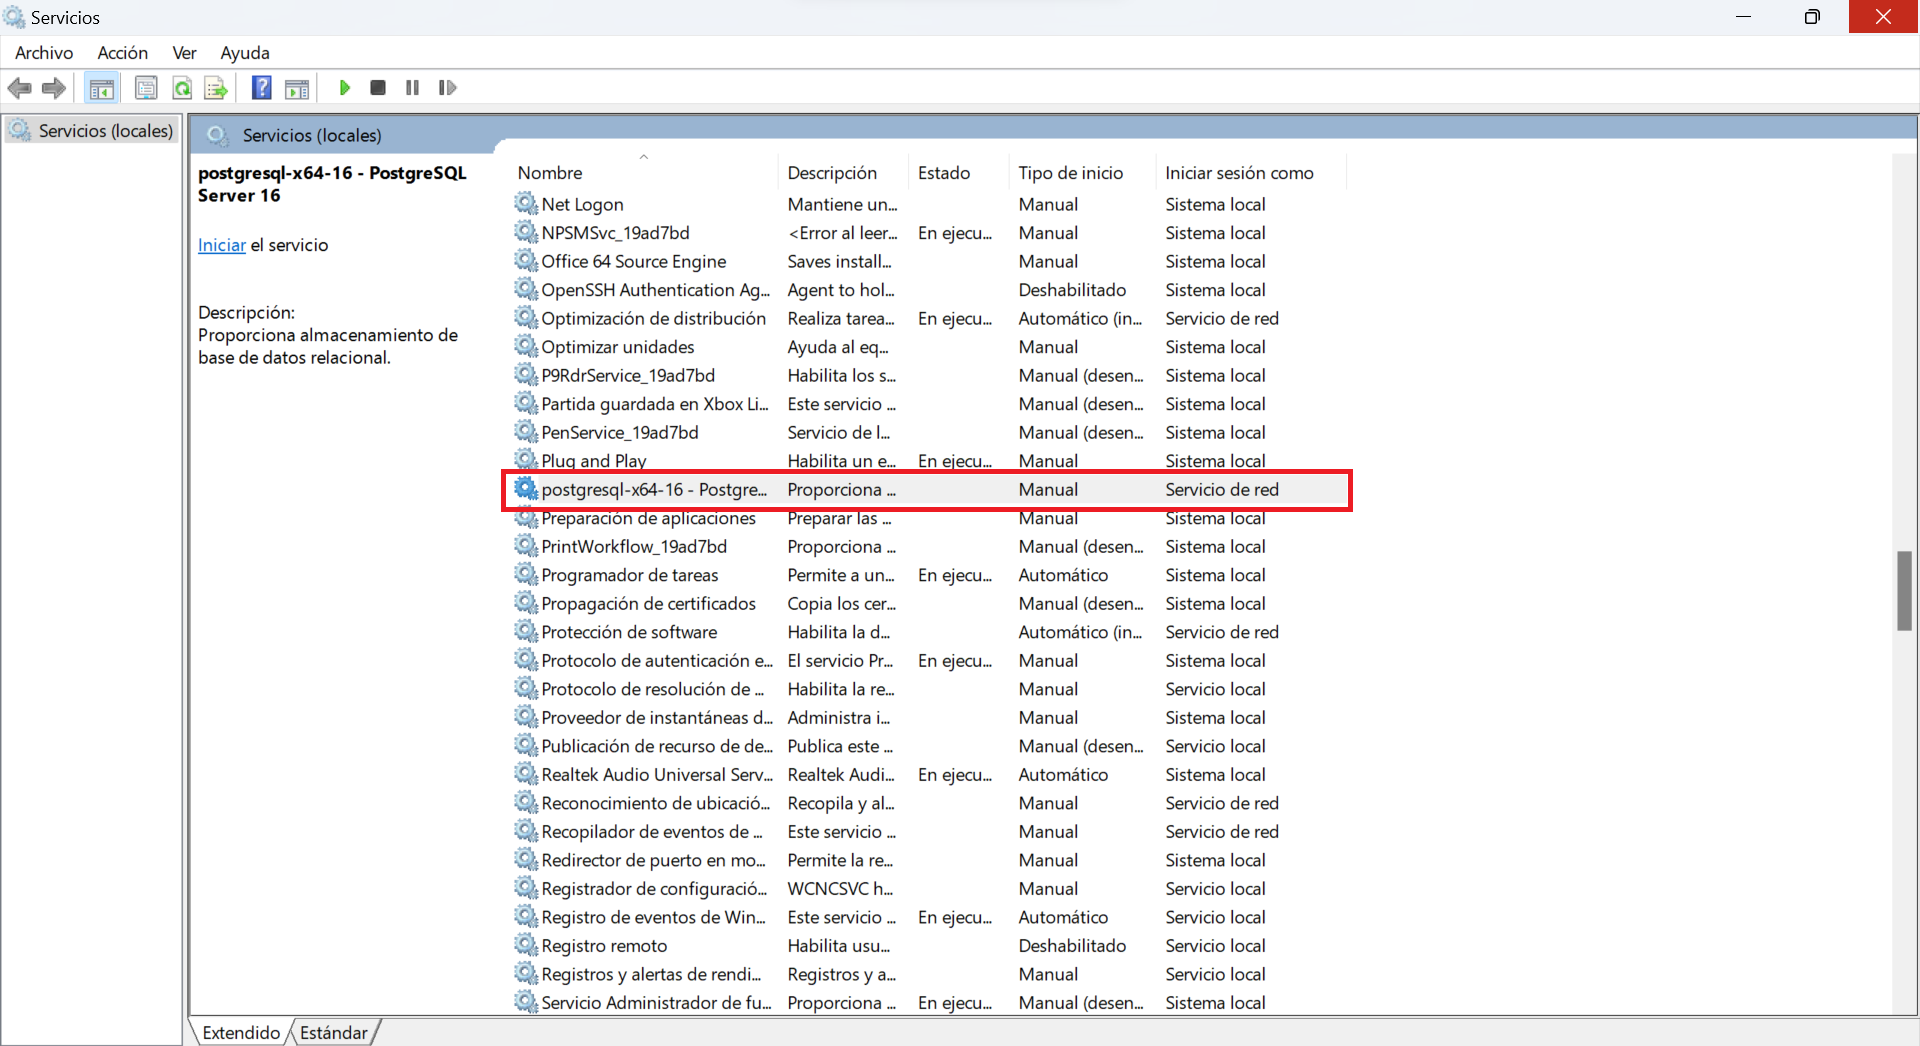
\includegraphics[width=0.90\textwidth]{figures/serviciosConfig.png}
     \caption{Captura de pantalla de la aplicación de servicios.}
    \label{fig:serviciosConfig}
    \end{figure}

    \item El último paso consiste en registrar el servidor a través del administrador de base de datos instalado en el equipo, en este caso pgAdmin. 
    
    Una vez que tengamos libre el puerto 5432, podemos registrar un nuevo servidor en dicho puerto que acceda a la base de datos de Broadsea. Para ello abrimos el administrador de la base de datos PostgreSQL, pgAdmin 4, y registramos un nuevo servidor. Los parámetros de configuración de este nuevo servidor se describen en el \textit{docker-compose.yml} y en la sección 3 del archivo \textit{.env}. Los parámetros fundamentales son:

    \begin{lstlisting}[language=sh]
        host = 127.0.0.1
        port = 5432
        user = postgres
        password = mypass\end{lstlisting}
    
    \item Tras registrar el servidor correctamente, debe aparecer una base de datos con cinco esquemas: \code{demo\_cdm}, \code{demo\_cdm\_results}, \code{public}, \code{webapi}, \code{webapi\_security}. Para comprobar que se ha establecido una conexión correcta con la base de datos, sin pérdida de información, se puede comprobar el número de filas que recupera pgAdmin de la tabla \code{person} del esquema \code{demo\_cdm}, tal y como se muestra en la Figura \ref{fig:pgAdmin}.

    \begin{figure}[H]
    \centering
    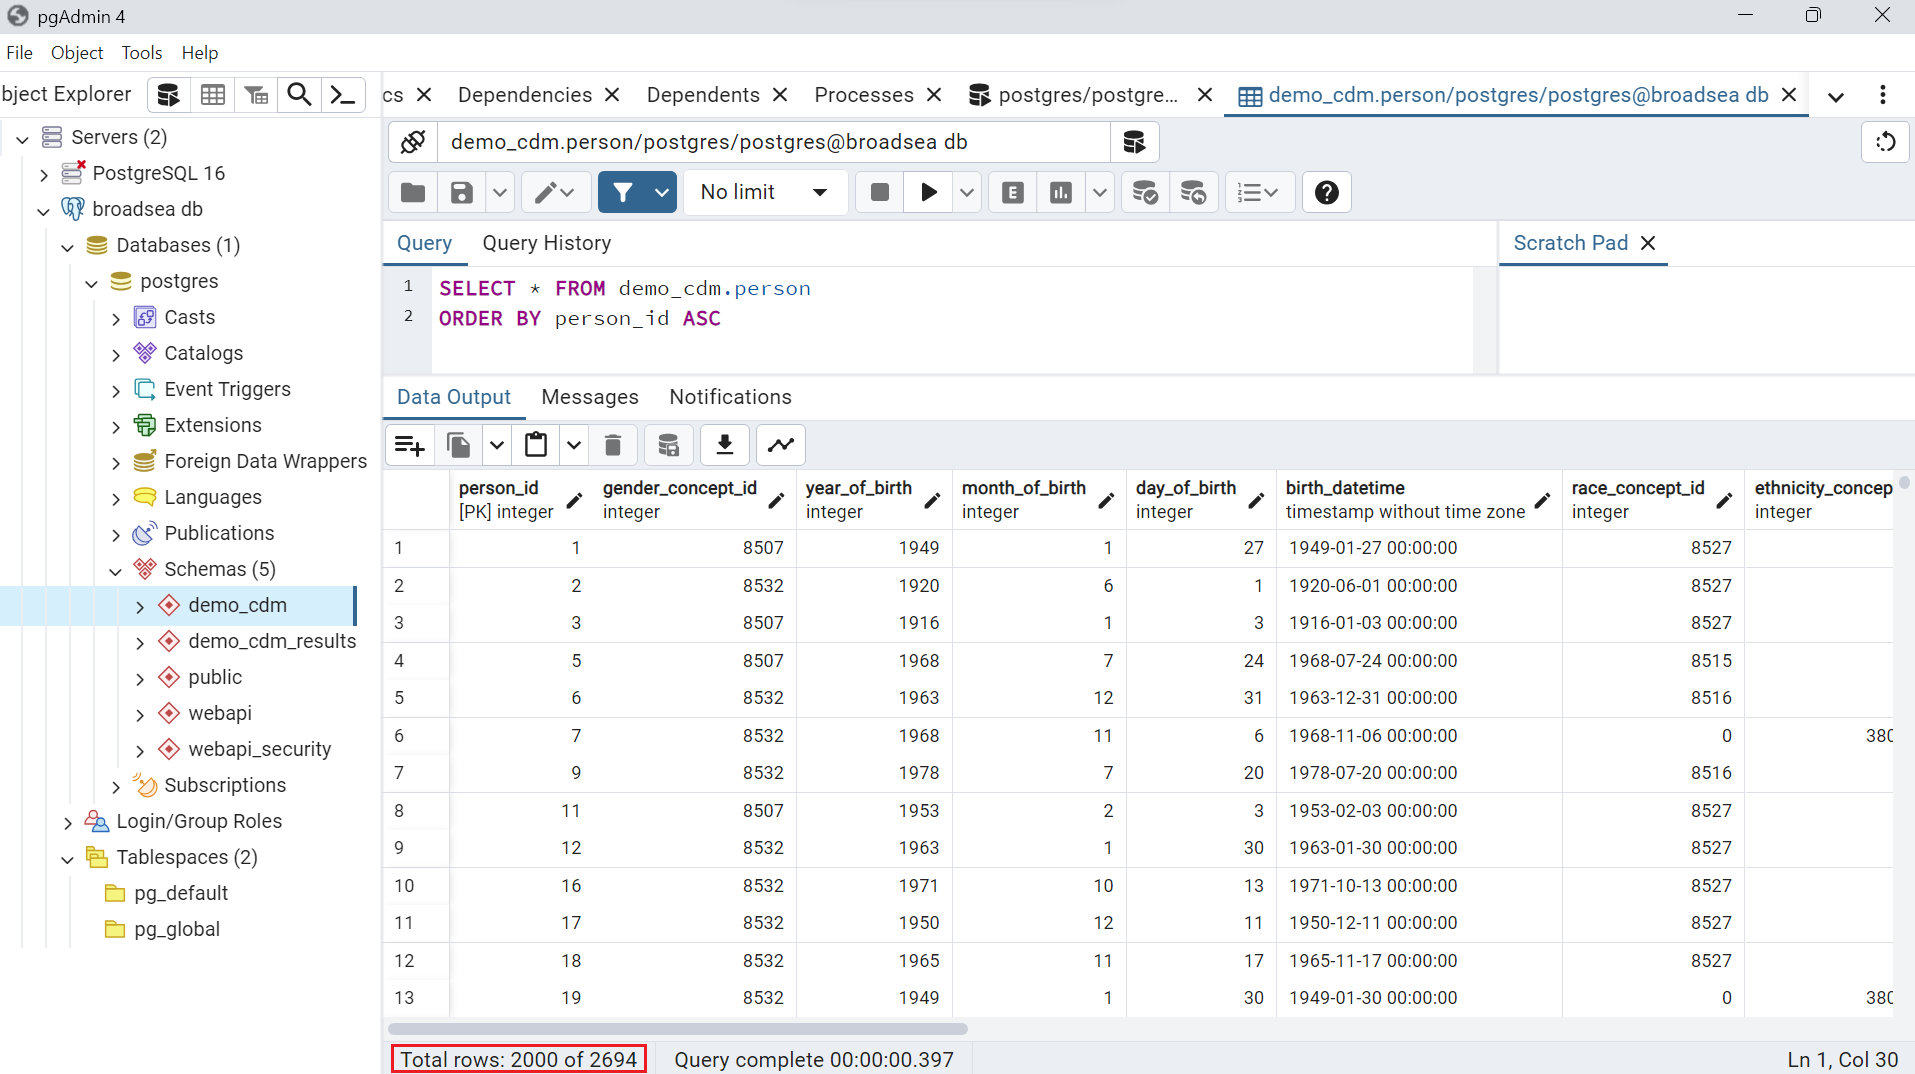
\includegraphics[width=0.90\textwidth]{figures/pgAdmin.png}
     \caption{Captura de pantalla de pgAdmin.}
    \label{fig:pgAdmin}
    \end{figure}

    El número de filas que recupere pgAdmin debe ser igual al número de personas que muestra ATLAS en la sección Data Sorce/Dashboard, en este caso son 2694 personas (Figura \ref{fig:dashboardEJ}).

    \begin{figure}[H]
    \centering
    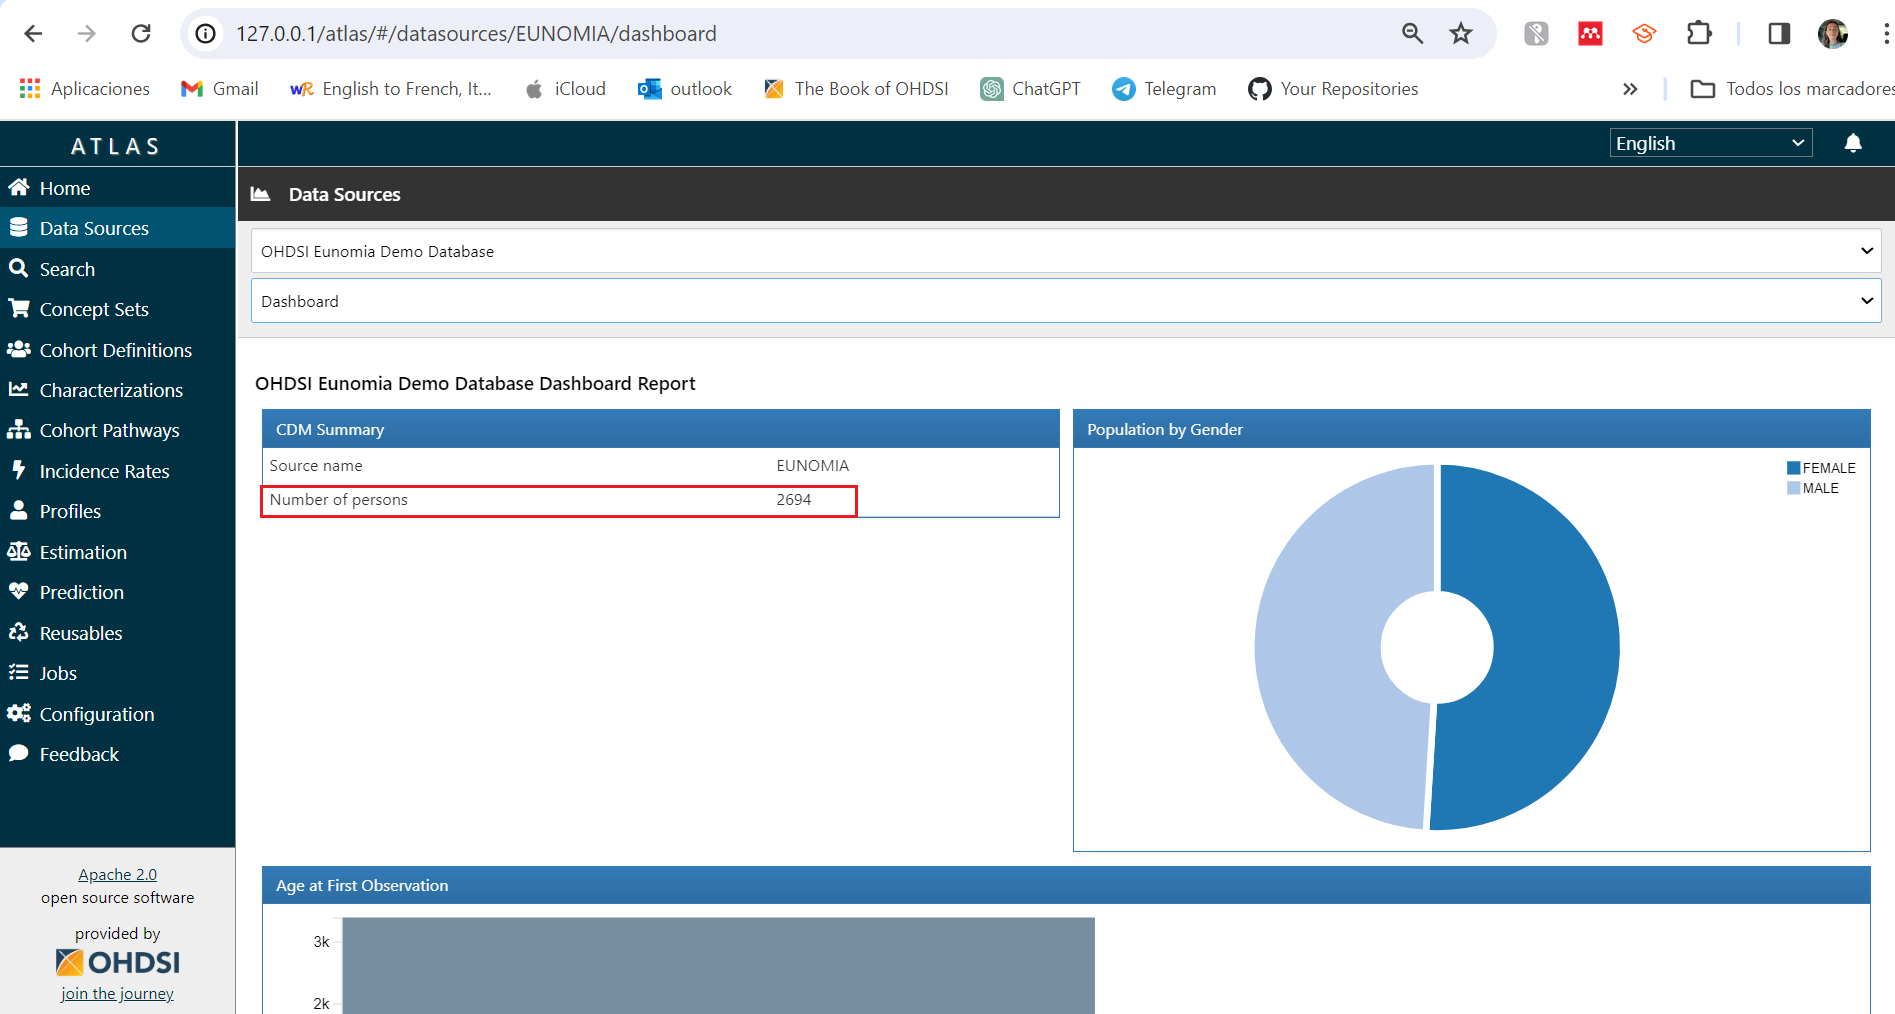
\includegraphics[width=0.90\textwidth]{figures/dashboardEJ.png}
     \caption{Captura de pantalla de ATLAS Data Sources/Dashboard.}
    \label{fig:dashboardEJ}
    \end{figure}

    \item Por último, otra forma de comprobar que la conexión es correcta y una forma alternativa de realizarla, con el fin de detectar posibles problemas durante la implementación, es ejecutar el siguiente script de código en R, que realiza la conexión con la base de datos a través de RStudio:

    \begin{figure}[H]
    \centering
    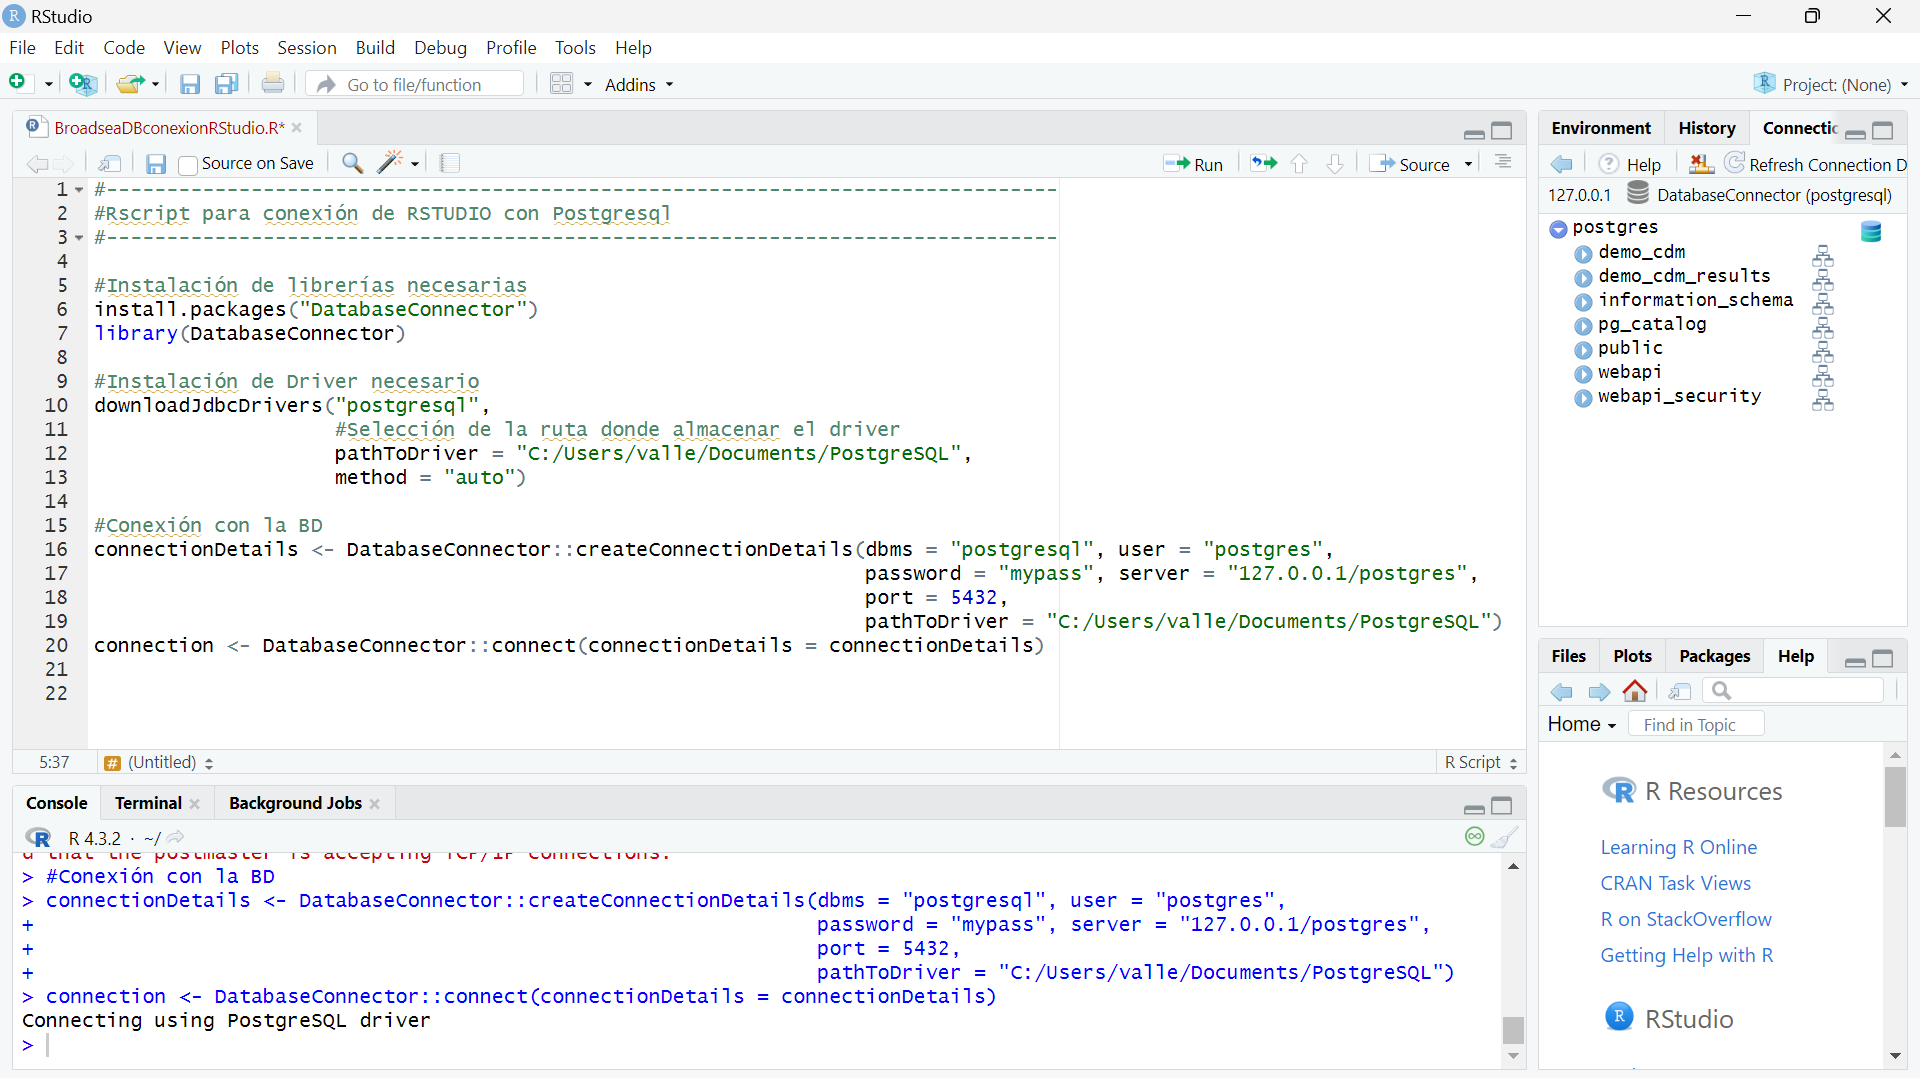
\includegraphics[width=0.90\textwidth]{figures/RStudio.png}
     \caption{Captura de pantalla de script de RStudio.}
    \label{fig:RStudio}
    \end{figure}
    
\end{enumerate}

\section{Solución de posibles problemas}

\subsubsection{Error: Connection timeout expired}
Al entrar en la base de datos de Eunomia e introducir la contraseña aparece el error.

    \begin{figure}[H]
    \centering
    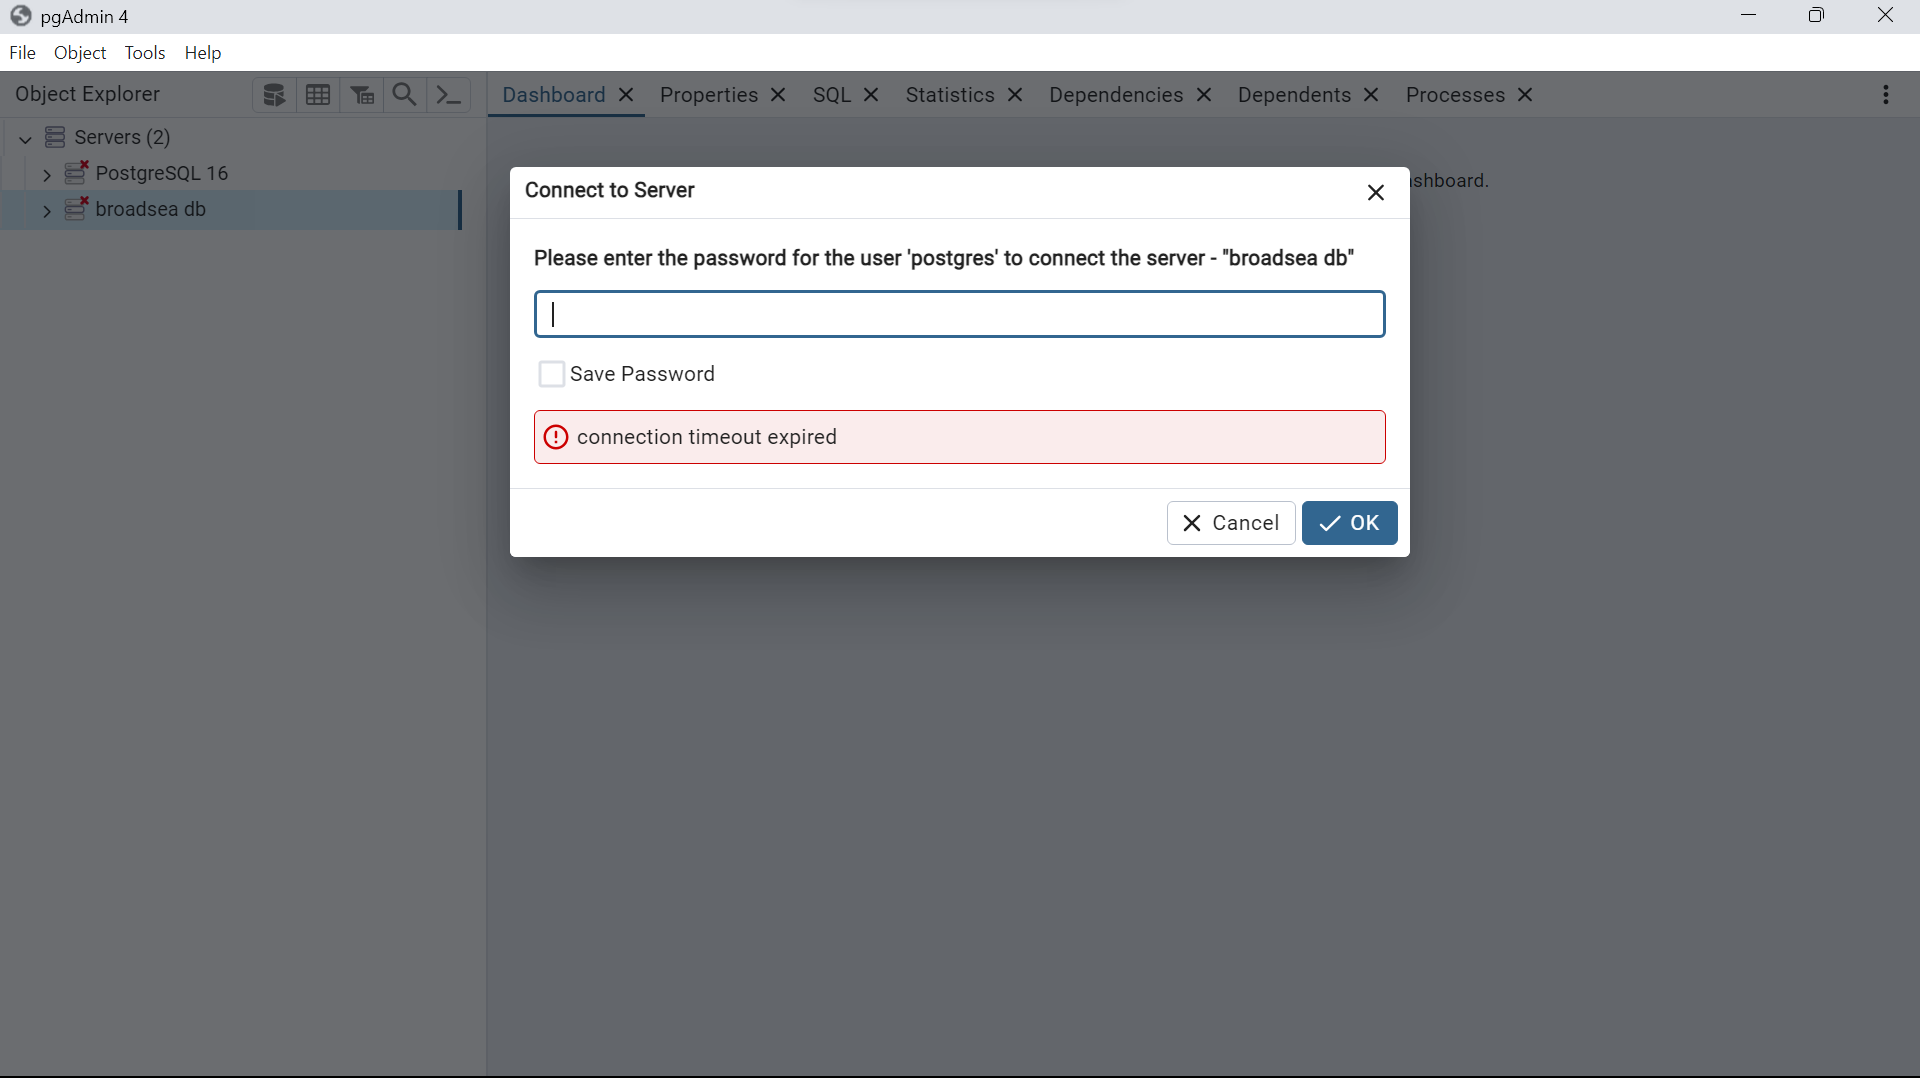
\includegraphics[width=0.90\textwidth]{figures/Error03ConnTime.png}
     \caption{Captura de pantalla de error.}
    \label{fig:Error03ConnTime}
    \end{figure}

Solución: Enciende el contenedor de docker.

\subsubsection{No permite establecer la conexión por puerto ocupado.}

 